\documentclass{book}
\usepackage{amsmath}
\usepackage{amssymb}

%maths
\usepackage{mathtools}
\usepackage{amsmath}
\usepackage{amssymb}
\usepackage{amsfonts}

%tikzpicture
\usepackage{tikz}
\usepackage{scalerel}
\usepackage{pict2e}
\usepackage{tkz-euclide}
\usetikzlibrary{calc}
\usetikzlibrary{patterns,arrows.meta}
\usetikzlibrary{shadows}

%pgfplots
\usepackage{pgfplots}
\pgfplotsset{compat=newest}
\usepgfplotslibrary{statistics}
\usepgfplotslibrary{fillbetween}

%colours
\usepackage{xcolor}

\usepackage{nicefrac}
\usepackage{geometry}
\geometry{
  a4paper, % or letterpaper
  top=1.5in,
  bottom=3in,
  left=2in,
  right=2in,
  headheight=14pt
}
\title{Calculus Math Notes}
\author{Alexys Ocegueda Castro}

\begin{document}

\pgfplotsset{
	standard/.style={
		axis line style = thick,
		trig format=rad,
		enlargelimits,
		axis x line=middle,
		axis y line=middle,
		enlarge x limits=0.15,
		enlarge y limits=0.15,
		every axis x label/.style={at={(current axis.right of origin)},anchor=north west},
		every axis y label/.style={at={(current axis.above origin)},anchor=south east}
	}
}

\maketitle
\tableofcontents

\chapter{Limits} Used in defining the important concepts in calculus such as continunity, derivative of a function, the definite integral of a function.
\section{What are Limits}
It's easy to brush off limits due to their inherent simplicity in solving for them, but it's good to know what is happening when you say a limit equals something. This means that as you zoom in on that one area it is \textit{approaching}, the number it equals, despite it potentially never reaching it, still is the answer. The limit is the number you inch closer and closer to while zooming in.\\

\subsection{Inituitive Definition}
The \textbf{limit} of a function describes the behavior of a function near a particular value of x.\\
\\
When a limit heads towards infinity due to a vertical asymptote this is said to be a \textbf{infinite limit}.\\

\section{One-Sided Limits}
When a limit has a '-' sign that means the limit as it approaches from the \textit{left}.\\
When a limit has a '+' sign that means the limit as it approaches from the \textit{right}.\\
\\

\section{Trigonometric Functions}
There are four important limit functions:\\
1. $\lim\limits_{x \to c} sinx = sinc$\\
2. $\lim\limits_{x \to c} cosx = cosc$\\
3. $\lim\limits_{x \to 0} \frac{sinx}{x} = 1$\\
4. $\lim\limits_{x \to 0} \frac{1-cosx}{x} = 0$

\section{Continunity}
Three conditions must be met for a point to considered continuous:\\
1.  f(c) exists\\
2. $\lim\limits_{x \to c} f(x)$\\
3. $\lim\limits_{x \to c} f(x) = f(c)$

\newpage
\begin{center}
	\begin{tikzpicture}
		\begin{axis}[standard,
			xtick={-7,...,6},
			ytick={-4,...,5},
			samples=1000,
			xlabel={$x$},
			ylabel={$y$},
			xmin=-7,xmax=6,
			ymin=-4,ymax=5,
			clip=false]

			\addplot[
				<->,
				thick,
				] {x+2} node[anchor=south] {c};

			\coordinate (P) at (axis cs: 2, 4); % Define a coordinate at the point (0, 2)
			\draw[thick,fill=white] (P) circle (3pt) node[right] {b}; % Draw a hollow circle centered at P
		
			\coordinate (Q) at (axis cs: 2, 1); % Define a coordinate at the point (0, 2)
			\draw[thick,fill=black] (Q) circle (3pt) node[right] {a}; % Draw a hollow circle centered at P
		
		\end{axis}
	\end{tikzpicture}
\end{center}

In the graph above we can say multiple things:\\
1. A limit exists at $f(b)$ which is 4.\\
2. The limit \textit{at} $f(b)$ is 1 aka 'a'.\\
3. This line has a disconnected continunity. \\
\\
A test would be to imagine a pencil going along $f(x)$ without having to be picked up -- if it can accomplish this then it is continuous.



\chapter{Derivatives}

\section{What is a Derivative}
It is the instantaneous rate of change which says how much something changes in relation to another. It's the slope of the tangent line at any given point revealing steepness and direction (increasing/decreasing). 

\subsection{Definition}
The derivative of a function $y = f(x)$ at point $(x, f(x))$, is defined as:
\begin{center}
  $\lim\limits_{\delta x \to 0} \frac{f(x + \delta x) - f(x)}{\delta x}$
\end{center}

Example: Using the definition, find the derivative of $f(x) = 5x - 4$\\
\\
You will want to add in delta into $f(x)$ when you utilize the definition.
\\
\begin{equation*}
  \begin{aligned}
    L &= \lim_{\Delta x \to 0} \frac{(5(x + \Delta x) - 4) - (5x - 4)}{\Delta x} \\
      &= \lim_{\Delta x \to 0} \frac{5x + 5\Delta x - 4 - 5x + 4}{\Delta x} \\
      &= \lim_{\Delta x \to 0} \frac{5\Delta x}{\Delta x} \\
      &= \lim_{\Delta x \to 0} 5 \\
      &= 5
  \end{aligned}
\end{equation*}

Note that \textbf{Differentiability implies continuity, but continuity \textit{does not} imply differentiability} 

\section{Differentiation Rules}
\begin{enumerate}
  \item If $f(x) = c$ where c is a constant, then $f'(x) = 0$.\\
  \item If $f(x) = c * g(x),$ then $f'(x) = c \cdot g'(x)$.\\
  \item Sum Rule: If $f(x) = g(x) + h(x)$ then $f'(x) = g'(x) + h'(x)$.\\
  \item Difference Rule: If $f(x) = g(x) - h(x)$, then $f'(x) = g'(x) - h'(x)$.\\
  \item Product Rule: If $f(x) = g(x) \cdot h(x)$, then $f'(x) = f(x)g'(x) + g(x)f'(x).$\\
  \item Quotient Rule: If $f(x) = g(x) / h(x)$, then $f'(x) = \frac{g'(x) \cdot h(x) - h'(x)g(x)}{[h(x)]^2}$
\end{enumerate}

\section{Trigonometric Functions}
The 6 trigonometric functions also have rules:
\begin{enumerate}
  \item$f(x) = sinx,$ then $f'(x) = cosx$\\
  \item $f(x) = cosx,$ then $f'(x) = -sinx$\\
  \item If $f(x) = tanx,$ then $f'(x) = sec^2x$\\
  \item If $f(x) = cotx,$ then $f'(x) = -csc^2x$\\
  \item If $f(x) = secx,$ then $f'(x) = secxtanx$\\
  \item If $f(x) = cscx,$ then $f'(x) = -cscxcotx$\\ 
\end{enumerate}

\subsection{Inverse Trigonometric Functions}
The 6 inverse trigonometric functions also have derivatives:\\
\begin{enumerate}
  \item If $f(x) = \sin^{-1}x = \arcsin x$\\
    $f'(x) = \frac{1}{\sqrt{1-x^2}}$\\
  \item If $f(x) = \cos^{-1}x = \arccos x$\\
    $f'(x) = \frac{-1}{\sqrt{1-x^2}}$\\
  \item If $f(x) = \tan^{-1}x = \arctan x$\\
    $f'(x) = \frac{1}{1+x^2}$\\
  \item If $f(x) = \cot^{-1}x = \arccot x$\\
    $f'(x) = \frac{-1}{1+x^2}$\\
  \item If $f(x) = \sec^{-1}x = \arcsec x$\\
    $f'(x) = \frac{1}{x\sqrt{x^2-1}}$\\
  \item If $f(x) = \csc^{-1}x = \arccsc x$\\
    $f'(x) = \frac{-1}{\sqrt{1-x^2}}$\\
\end{enumerate}

\section{Chain Rule}
The \textbf{chain rule} is a technique for finding the derivative of composite functions. With the number of differentiation steps dependent on how many functions there are. \\
\\Example 1:\\ $f(x) = (g \circ h)(x) = g[h(x)]$ then \\
$f'(x) = g'[h(x)] \cdot h'(x)$
\\\\
Example 2:\\$r(x) = (m \circ n \circ p)(x) = m\{n[p(x)]\}$\\
then $r'(x) = m'\{n[p(x)]\} \cdot n'[p(x)] \cdot p'(x)$

\section{Differentiation of Exponential and Logarithmic Functions}
Here are their differentiations formulas:\\
\begin{enumerate}
\item If $f(x) = e^x,$ then $f'(x) = e^x$.\\
\item If $f(x) = a^x, a > 0, a \neq 1$, then $f'(x) = (\ln a)\cdot a^x$.\\
\item If $f(x) = \ln x$, then $f'(x) = \frac{1}{x}$.\\
\item If	$f(x) = \log_{a} x, a > 0, a \neq 1, then f'(x) = \frac{1}{(\ln a)\cdot x} $.
\end{enumerate}

\newpage
\section{Implicit Differentiation}
Implicit Differentiation allows you to find the derivative of y with respect to x without having to solve the given equation for y.
\\\\
Example: Find $y'$ when $y = \sin x + \cos y$
\begin{equation*}
  \begin{aligned}
    y' &= \cos x - \sin y \cdot y' \\
    y' + \sin y \cdot y' &= \cos x  \\
    y'(1 + \sin y)    &= \cos x \\
    y' &= \frac{\cos x}{(1 + \sin y)} \\
  \end{aligned}
\end{equation*}

\section{Higher Order Derivative}
The degree of derivative depends on how many successive derivatives where taken which are called \textbf{higher order derivative}.\\
\\
\noindent \textbf{Example:} Find the second derivative of $f(x) = 20x^3 - 9x^2 + 3x + 2$.

\begin{equation*}
  \begin{aligned}
    f'(x)  &= 60x^2 - 18x + 3 \\
    f''(x) &= 120x - 18
  \end{aligned}
\end{equation*}


%\chapter{Exponential and Logarithmic Functions}
Explores exponential growth and decay, graphing exponential functions, defining and using logarithms, and solving equations involving exponents and logarithms.

\section{Exponential and Logarithmic Functions}
\subsection{Exponential Functions}
Any function defined by $y = b^x$, where $b > 0, b \ne 1$, and x is a real number, is called an exponential function.\\

\subsection{Logarithmic Functions}
if $x = 2^y$ were to be solved for y then you'd be finding the \textbf{logarithm}.\\
\\
Common Logarithms are ones with base 10.\\
Natural Logarithms are ones with base e.\\


%\chapter{Factoring Polynomials}


\section{Factoring Polynomials}
\textbf{Factoring} is when you rewrite a polynomial as a product of polynomials.\\

\subsection{Greatest Common Factor}
The first method is called \textbf{greatest common factor} as you factor out the largest number in the polynomial.\\
\\
Example: $5x + 5y = 5(x + y)$\\

\subsection{Difference of Squares}
The product of conjugates produces a pattern called a \textbf{difference of squares}.\\
\\
Example: $(a + b)(a - b) = a^2 - b^2$\\
\\

\subsection{Sum or Difference of Cubes}
\textbf{Sum of Cubes} is the form $(a)^3 + (b)^3$.\\
\textbf{Difference of Cubes} is the form of $(a)^3 - (b)^3$\\
\\
They have similar factored patterns where they follow the same rules.\\
The first binomial has the same sign, but the trinomial has the \textit{opposite} sign.\\
$(a)^3 + (b)^3 = [(a) + (b)][(a)^2 - (a)(b) + (b)^2]$\\
\\
$(a)^3 - (b)^3 = [(a) + (b)][(a)^2 + (a)(b) + (b)^2]$\\


\textbf{Trinomials of the Form $x^2 + bx + c$}
Example: $2x^2 + 16x + 24$ \\
\\
Step 1: See if you can take out the Greatest Common Factor to make the problem easier. In this case you can take out a \textit{2} from all three numbers.

To factor these you first distribute the first $x^2$ into two parenthesis to start:\\ Don't forget to put the 2 you factored out in the beginning. So far we have $2(x^2 + 8x + 12)$.
	$2(x )(x )$\\
\\
Now you think of two numbers which can add up the middle number but also multiply to the last number. Keep in mind you can switch up the symbols to make either one positive or negative. Some factors to try are:
$(1)(12)$, $(-1)(-12)$, $(2)(6)$, $(3)(4)$\\
\\
Plugging in 2 and 6 we can see that they add up to 8 and multiply to 12 giving us our factored trinomial, which keep in mind is just two binomial.\\
\\
$2(x + 2)(x + 6)$\\
\\
\subsection{Sqaure Trinomials}
Recall $(x + y)^2 = (x)^2 + 2(x)(y) + (y)^2$\\
\\
Therefore, it is easy to see if an equation is a square trinomial or binomial.\\
\\
Example: $4x^2 - 20x + 25$ can be deduced down to squares: $4x^2 = (2x)^2$ \& $25 = (-5)^2$\\
Leaving us with the final step of putting them in the form $2xy$ to see if it fits: 2(2x)(-5) which does equal -20x like the original equation. This means $(2x - 5)^2$ is the square binomial to our original trinomial.\\
\\

\subsection{Factoring by Regrouping}
There are two main things to look for in attempting to factor a polynomial of four or more terms with no GCF. It can be regrouped into two groups of two terms or two groups where one has three terms aka a trinomial. \\
\\
Example: (az + ay) + (bz + by)\\
\\
We can factor out both an 'a' and a 'b'. Leaving us with $a(y + z) + b(y + z)$. Now we see we can see that we can factor out (y + z) leaving us now with $(y + z)(a + b)$. \\


%\documentclass{article}
\usepackage{graphicx} % Required for inserting images
\usepackage{tikz}

% \title{Geometry}
% \author{Alex Ocegueda}
% \date{October 2025}

\begin{document}

% \maketitle

\section{Linear equations}
\textbf{Linear Equation} is one variable with the exponent 1 in an equation. Also known as first degree equations.\\
\textbf{Formulas} are equations that describes a relationship between unknown values.\\
\\
\begin{equation}\label{perimeter} 
	Perimeter = 2l + 2w\\
\end{equation}

\begin{equation}\label{trapezoid} 
	Trapezoid = \frac{1}{2}h(b_1 + b_2)\\
\end{equation}

\begin{equation}\label{ratedistance} 
	RateDistance = \frac{D}{T} = R\\
\end{equation}

\begin{equation}\label{accumulatedinterest} 
	Accumulated Interest = \frac{A - P}{PR} = T\\
\end{equation}

\begin{equation}\label{absolutevalue} 
	absolutevalue_1 = |A| + |-A| = A + A
\end{equation}

\subsection{Linear Inequalities}
\textbf{inequality} is a sentence using symbols other than equality
\\
\subsection{Compound Equalities}
\textbf{Compound Inequality} is a sentence with two inequality statements


\end{document}

%\include{linear-sentence-two-vars/two-vars}
%\chapter{Polynomial Arithmetic}

\section{Polynomial Arithmetic}

\subsection{Adding and Subtracting Polynomials}
\textbf{Monomial} is an expression that could be a numeral, a variable, or the product of numerals and variables within certain restrictions.\\
\\
1. Must have whole number exponents.\\
2. Variables do not appear under simplified radical expressions.\\
3. Denominators do not contain variables.\\

\textbf{Examples:} $-10$, $a$, $5t^2$, $3/8x^2y^3$ \\
\\
\textbf{Binomial} is an expression that is the sum of two monomials.\\
\textbf{Trinomial} is an expression that is the sum of three monomials.\\
\textbf{Polynomial} is an expression that is a monomial or the sum of two or more monomials.\\
\\

\subsection{Multiplying Polynomials}
1. $x^ax^b = x^{a+b}$ \\Multiplying monomials with the same base you keep the base and add the powers.\\\\
2. $(x^a)^b = x^{ab}$\\ Keep the base and multiply the powers when finding powers of a base.\\\\
3. $(xy)^a = x^ay^a$ \\Raise each factor in the proudct to the power when finding the powers of a product\\\\

\subsection{Special Products of Binomials}
\textbf{Conjugates} are two binomials with the same two terms but opposite signs separating the terms. They are conjugates of each other.\\
\\Example: $3x + 2$ \& $3x - 2$\\

\textbf{Difference of Squares} is the \textit{product} of conjugates which produces a special pattern.\\
\\Example: $(x + y)(x - y) = x^2 - y^2$\\
\\
\textbf{Square Trinomial} is the pattern produced by squaring a binomial.\\
\\Example: $(x + y)^2 = x^2 + 2xy + y^2$ \& $(x - y)^2 = x^2 - 2xy + y^2$\\
\\
Notice how only the \textit{first} sign is changed when subtracting a squared binomial.
\\ \\

\subsection{Dividing Polynomials}
\begin{center}
	\framebox{$a^m/a^n = a^{m-n}$} \\
\end{center}
This works as long as a does not equal zero.\\
\\
\begin{center}
	\framebox{$a^-n = 1/a^n$ \& $1/a^-n = a^n$} \\
\end{center}
This works as long as \textit{a} does not equal zero.\\ Also works in reverse.
\\

\subsection{synthetic Division}
\textbf{Synthetic Division} is a shortcut for polynomial division when the divisor is the form of x-a. Only the coefficients are used when dividing.\\
\\
Example: Divide $(3x^2 + 2x - 11)$ by $(x-3)$\\
\\
First step would be multiplying $(x-3)$ by $3x^2$ giving you $3x^3 - 9x^2$. You subtract this and keep repeating until you are left with a remainder. The remainder is added at the end by being divided by the divisor.


%\documentclass{article}

%maths
\usepackage{mathtools}
\usepackage{amsmath}
\usepackage{amssymb}
\usepackage{amsfonts}

%tikzpicture
\usepackage{tikz}
\usepackage{scalerel}
\usepackage{pict2e}
\usepackage{tkz-euclide}
\usetikzlibrary{calc}
\usetikzlibrary{patterns,arrows.meta}
\usetikzlibrary{shadows}

%pgfplots
\usepackage{pgfplots}
\pgfplotsset{compat=newest}
\usepgfplotslibrary{statistics}
\usepgfplotslibrary{fillbetween}

%colours
\usepackage{xcolor}

\usepackage{nicefrac}

\begin{document}

\section{Polynomial Functions}
A \textbf{Polynomial Function} is any function of the form:\\
\begin{center}
	$a_0x^n +a_1x^{n-1}  +a_2x^{n-2} +...+ a_{n-1}x+ a_n$ 
\end{center}

\subsection{Zeros of a Function}
\textbf{Zeros of a Function} is when you make a function equal zero so you can find the roots which equal zero. This tells you the x-intercepts of the graph. \\
\\
\end{document}

%\chapter{Quadratics in One Variable}

\section{Quadratics in One Variable}
A \textbf{Quadratic Equation} is any equation of the form:\\

\begin{center}
	$ax^2 + bx + c = 0$ (a \ne 0)
\end{center}
\\\\
You can solve them in 4 ways:\\
1. Factoring\\
2. Applying Square Root property\\
3. Completing the square\\
4. Applying the quadratic formula\\


%\documentclass{article}

%maths
\usepackage{mathtools}
\usepackage{amsmath}
\usepackage{amssymb}
\usepackage{amsfonts}

%tikzpicture
\usepackage{tikz}
\usepackage{scalerel}
\usepackage{pict2e}
\usepackage{tkz-euclide}
\usetikzlibrary{calc}
\usetikzlibrary{patterns,arrows.meta}
\usetikzlibrary{shadows}

%pgfplots
\usepackage{pgfplots}
\pgfplotsset{compat=newest}
\usepgfplotslibrary{statistics}
\usepgfplotslibrary{fillbetween}

%colours
\usepackage{xcolor}

\usepackage{nicefrac}

\begin{document}
\section{Radicals and Complex Numbers}

\textbf{Radical Expression} is the form $\sqrt[n]{a}$. The $\sqrt{}$ is a radical sign and the expression under it is the \textit{radicand}, while the $n$ is called the \textit{index}.
\begin{center}
	\fbox{If $x = \sqrt[n]{a}$, then $x^n = a$}
\end{center}

\subsection{Adding and Subtracting Radical Expressions}

Radical expressions are called \textbf{like radical expressions} if the indexes and radicands are the same. \\
\\
Example: $3\sqrt{7} + 5\sqrt{7} = 8\sqrt{7}$

\subsection{Multiplying Radical Expressions}
To multiply we simply distribute each one then add them.\\
\\
\subsection{Dividing Radical Expressions}
To divide we simply apply the sqrt to both top and bottom.\\
\\
\subsection{Rational Exponents}
if n is a natural number greater than 1, and b is any nonnegative real number, then:\\
\\
\begin{center}
	$b^{1/n}=\sqrt[n](b)$
\end{center}

\subsection{Complex Numbers}
Imaginary values and pure imaginary numbers. The expression $\sqrt{-1}$ has no real answer. The symbol for it is \textit{i} because its called an imaginary value. Any expression that is a product of a real number with i is called a pure imaginary number. \\
\\
\begin{center}
	$i = \sqrt{-1}$, $ i^2 = -1$
\end{center}
\end{document}

%\documentclass{article}

%maths
\usepackage{mathtools}
\usepackage{amsmath}
\usepackage{amssymb}
\usepackage{amsfonts}

%tikzpicture
\usepackage{tikz}
\usepackage{scalerel}
\usepackage{pict2e}
\usepackage{tkz-euclide}
\usetikzlibrary{calc}
\usetikzlibrary{patterns,arrows.meta}
\usetikzlibrary{shadows}

%pgfplots
\usepackage{pgfplots}
\pgfplotsset{compat=newest}
\usepgfplotslibrary{statistics}
\usepgfplotslibrary{fillbetween}

%colours
\usepackage{xcolor}

\usepackage{nicefrac}

\begin{document}

\section{Rational Expressions}
The quotient of two polynomials is called a \textbf{rational expression}, where the denominator is never zero.\\
\\
Examples include $5/6$, $\frac{3x + 8}{2x - 9}$, $6x + 5$\\
\\
The last one can be written as $\frac{6x + 5}{1}$ which fits the definition.

\subsection{Simplifying Rational Expressions}
1. Completely factor numerators and denominators.
2. Reduce common factors.\\
\\
\subsection{Multiplying Rational Expressions}
1. Completely factor all numerators and denominators.\\
2. Reduce all common factors.\\
3. Either multiply the denominators, using FOIL if needed, or leave it in factored form.\\
\\
\subsection{Dividing Rational Expressions}
Division of fractions involves multiplying by the \textit{reciprocal} of the divisor.

\subsection{Adding and Subtracting Rational Expressions}
If they have the same denominator then add/subtract as usual making sure to simplify at the end.\\
If they \textit{dont} have the same denominator then you need to find the Lowest Common Denominator (LCD).\\

\subsection{Complex Fractions}
If the numerator or denominator or both contain fractions the expression is called a \textbf{complex fraction.}\\
\\
1. Simplify both numerator and denominator expressions into single fraction expressions.\\
2. Divide the numerator by the denominator and simplify if possible.\\
\\

\subsection{Proportion, Direct Variation, Inverse Variation, Joint Variation}
\textbf{Proportion} is an equation stating that two rational expressions are equal. Simple ones are solved with the \textit{Cross Product Rule}\\
\\
\[
\fbox{
    \parbox{4cm}{ % You need to set a width for the parbox
        \textbf{Cross Product Rule} \\ 
        if $\frac{a}{b} = \frac{c}{d}$, then $ad = bc$.
    }
}
\]
\textbf{Direct Variation} is when 'y varies directly as x' or 'y is directly proportional to x'. This may be inteperted in two ways:\\
\\
1. $\frac{y}{x} = k $ \\
\\
For some constant k - k is called the \textbf{constant of proportionality}. This is used when the constant is the desired result.\\
\\
2. $\frac{y_1}{x_1} = \frac{y_2}{x_2}$ \\
\\
This is when the desired result is either an original or new value of x or y.\\
\\

\textbf{Inverse Variation} is when 'y varies inversely (opposite) to x'.

\textbf{Joint Variation} is when one variable varies as the product of the other variables. The phrase goes 'y varies jointly as x and z':\\
\\
1. $\frac{y}{xz} = k$ \\
\\
if the constant is desired.\\
\\
2. $\frac{y_1}{x_1z_1} = \frac{y_2}{x_2z_2}$\\
\\
if one of the variables is desired.\\
\\


\end{document}

%\documentclass{article}

%maths
\usepackage{mathtools}
\usepackage{amsmath}
\usepackage{amssymb}
\usepackage{amsfonts}

%tikzpicture
\usepackage{tikz}
\usepackage{scalerel}
\usepackage{pict2e}
\usepackage{tkz-euclide}
\usetikzlibrary{calc}
\usetikzlibrary{patterns,arrows.meta}
\usetikzlibrary{shadows}

%pgfplots
\usepackage{pgfplots}
\pgfplotsset{compat=newest}
\usepgfplotslibrary{statistics}
\usepgfplotslibrary{fillbetween}

%colours
\usepackage{xcolor}

\usepackage{nicefrac}

\begin{document}

\pgfplotsset{
	standard/.style={
		axis line style = thick,
		trig format=rad,
		enlargelimits,
		axis x line=middle,
		axis y line=middle,
		enlarge x limits=0.15,
		enlarge y limits=0.15,
		every axis x label/.style={at={(current axis.right of origin)},anchor=north west},
		every axis y label/.style={at={(current axis.above origin)},anchor=south east}
	}
}

\section{Relations And Functions}

\textbf{Relation} is a set of ordered pairs that can be represented by a diagram, graph, or sentence.\\
\\
The \textbf{Domain} is the set of all \textit{first} numbers of the ordered pairs in a relation.\\
The \textbf{Range} is the set of all \textit{second} numbers of the ordered pairs in a relation. \\
\\
A \textbf{Function} is when none of the domain values are repeated.\\
A \textbf{Vertical Line Test} is a test for functions.\\
\\
\subsection{Compositions of Functions}
A \textbf{composite function} is when a variable is replaced with another function.\\
\\
Example: f(g(x)) is read as: 'f of g of x'\\
\\
\textbf{Inverse Relations} is when you reverse ordered pairs of an initial relation.\\
The \textbf{identity function} is the line which if you folded the graph over on this line/crease it would line up both relations. Since for each replacement of x, the result is identical to x.

\begin{center}
	\begin{tikzpicture}
		\begin{axis}[standard, 
			xtick={-4,-3,-2,-1,0,1,2,3,4,5,6,7,8},
			ytick={-4,-3,-2,-1,0,1,2,3,4,5,6,7,8},
			samples=1000,
			xlabel={$x$},
			ylabel={$y$},
			xmin=-4,xmax=8,
			ymin=-4,ymax=8,
			clip=false]

			% horizontal line - a
			\addplot[
				<->,  
				thick, 
				domain=-4:8,
				samples=2
				] {x} node[anchor=south] {$y=x$};

			\fill (2,1) circle (2pt);
			\fill (1,2) circle (2pt);
			\fill (6,4) circle (2pt);
			\fill (4,6) circle (2pt);
			\fill (8,3) circle (2pt) node[anchor=south] {$R^{-1}$};
			\fill (3,8) circle (2pt) node[anchor=south] {$R$};






		\end{axis}
	\end{tikzpicture}
\end{center}

\end{document}

%\chapter{Coordinate System}
\section{Rectangular Coordinate System}
\textbf{Coordinates of a point} is how each point on a plane is assigned a pair of numbers.\\
\textbf{Origin} is the point of \textit{intersection} of the x-axis and y-axis.\\
\textbf{Coordinate Plane} is the x-axis, y-axis, and all the points in their plane.\\
\textbf{Ordered Pairs} is a pair of numbers, written in parethesis and separated by comma for a point. Every point on a coordinate plane determined by order of numbers. example being (0,0) for the origin.\\
\textbf{X-Coordinate} is the number to the left of the comma in an ordered pair and determines the movement along the x-axis from origin. It moves right for positive and left for negative.\\
\textbf{Y-Coordinate} is the number to the right of the comma in an ordered pair and determines the movement perpendicular from the x-coordinate. It moves above the x-coordinate for positive and below the x-coordinate for negative.
\\
\textbf{Quadrants} are the four separated regions of a coordinate plane. Starting on top right and going counter-clockwise they're are named Quadrant I-IV.\\
\textbf{Graph} is the point associated with an ordered pair of real numbers.

\subsection{Distance Formula}
\begin{center}
	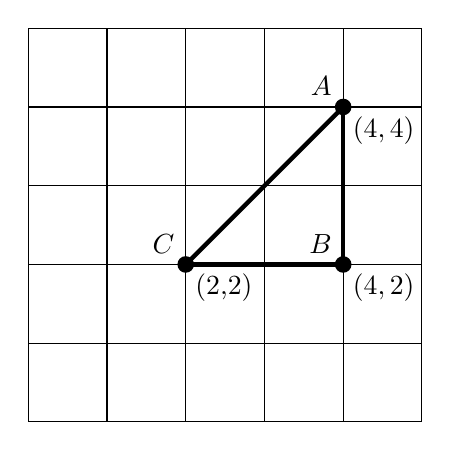
\begin{tikzpicture}
		\draw (0,0) grid (5,5);
		\draw[ultra thick] (2,2) -- (4,2) node[above left] {$B$};\fill (2,2) circle (3pt) node[below right] { (2,2) };
		\draw[ultra thick] (4,2) -- (4,4) node[above left] {$A$};\fill (4,2) circle (3pt) node[below right] {$(4,2)$};
		\draw[ultra thick] (4,4) -- (2,2) node[above left] {$C$};\fill (4,4) circle (3pt) node[below right] {$(4,4)$};
	\end{tikzpicture}

\end{center}

\begin{equation}
	d = \sqrt{(x_2 - x_1)^2 + (y_2 - y_1)^2}	
\end{equation}

All distances can be found by subtracting, except the \textit{hypotenuse}, which is found using the \textbf{Pythagorean Formula}.

\subsection{Midpoint Formula}
\begin{center}
	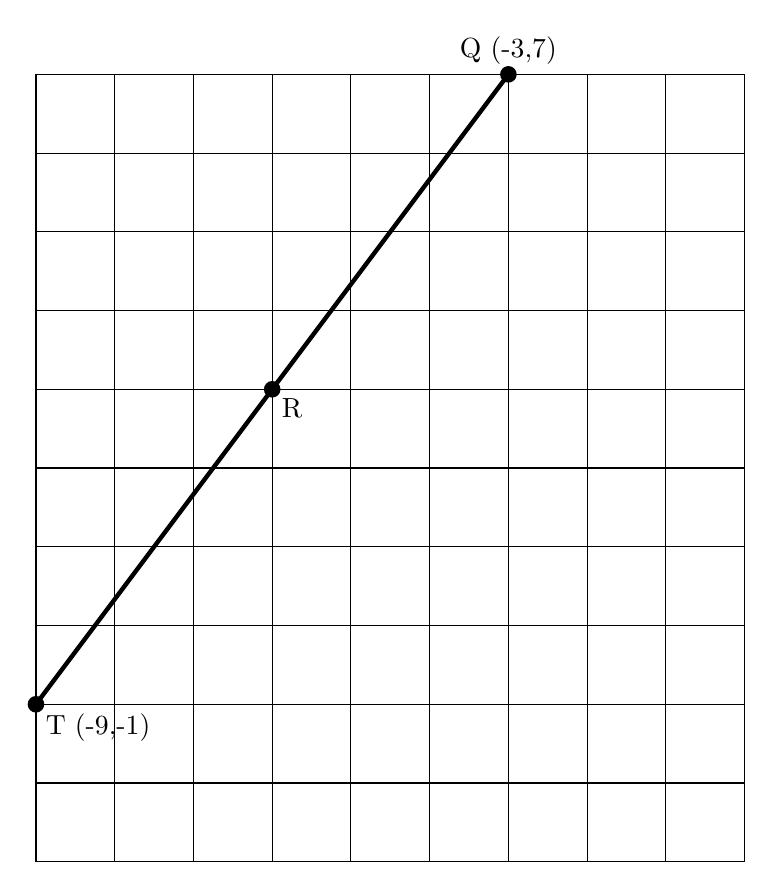
\begin{tikzpicture}
		\draw (-9,-3) grid (0,7);
		\draw[ultra thick] (-9,-1) -- (-3,7); \fill (-9,-1) circle (3pt) node[below right] {T (-9,-1) };
		\fill (-3,7) circle (3pt) node[above] {Q (-3,7)};
		\fill (-6,3) circle (3pt) node[below right] {R};
	\end{tikzpicture}
\end{center}

\begin{equation}
	M = (\frac{x_1 + x_2}{2},\frac{y_1 + y_2}{2})
\end{equation}

\textbf{Midpoint} is the average of the endpoints.

\newpage
\subsection{Slope of a Line}

\begin{center}
	\begin{tikzpicture}
		\begin{axis}[standard, 
			xtick={-7,-6,-5,-4,-3,-2,-1,0,1,2,3,4,5,6},
			ytick={-4,-3,-2,-1,0,1,2,3,4,5},
			samples=1000,
			xlabel={$x$},
			ylabel={$y$},
			xmin=-7,xmax=6,
			ymin=-4,ymax=5,
			clip=false]

			% horizontal line - a
			\addplot[
				<->,
				blue,  
				thick, 
				domain=-7:6,
				samples=2
				] {3} node[anchor=south] {$a$};

			\addplot[
				<->,
				gray,  
				thick
				] coordinates {(-2, -4) (-2, 5)} node[anchor=south] {b};

			\addplot[
				<->,
				thick,
				] {x+2} node[anchor=south] {c};

		\end{axis}
	\end{tikzpicture}
\end{center}
\[
	\boxed{m = \dfrac{y_2 - y_1}{x_2 - x_1}}
\]

The \textbf{slope of a line} is a measurement of steepness and direction of a \textit{nonvertical} line. This means line \textbf{b} has an undefined slope, while slope \textbf{a} has a slope of 0.
Meanwhile, \textbf{c} has an x-intercept at -2 and a y-intercept at 2. These intercepts are when either x or y are equal to 0.

\newpage
\subsection{Slopes of Parallel and Perpendicular Lines}
\textbf{Parallel} lines have equal slopes and \textbf{Perpendicular} lines have \textit{opposite} slopes/their product is -1. \\

\textbf{Example:} 
Given the original slope:
$$m = \frac{3}{4}$$

The slope of a parallel line ($m_{\parallel}$) is the same:
$$m_{\parallel} = \frac{3}{4}$$

The slope of a perpendicular line ($m_{\perp}$) is the negative reciprocal:
$$m_{\perp} = -\frac{4}{3}$$

\subsection{Equations of Lines}
\textbf{1.} If a point lies on the graph of an equation, then its coordinates make the equation true, and \\\\
\textbf{2.} If the coordinates of a point make an equation a true statement, then the point lies on the graph of the equation.

They can be written in the form of Ax + By = C, where A \& B are not zero. If they were zero then C would always have to be zero too making the form false.

\textbf{Standard Form} is $Ax + By = C$ for the equation of a line. \\
\textbf{X-Intercept} is where the y-coordinate is 0. \\
\textbf{Y-Intercept} is where the x-coordinate is 0. \\

\textbf{Note:} Horizontal lines have no x-intercept unless its on the x-axis.\\Vertical lines have no y-intercept unless its on the y-axis.

\subsection{Graphs of Linear Inequalities}
\textbf{Linear Inquality} is a sentence in the form of $Ax + By < C$. This can be any less than, greater than, or less/greater than or equal to symbol.
\\\\
If it is 'or equal to' then you make the line solid when graphing.\\ If it is not, then you make the line dotted as a boundary. This is because you are not counting what is on the line. 
\\\\
Now you want to plot a test point that is \textit{not} on the line. If this test point is true for the inequality then shade the side it is on, if not, shade the opposite side if it is false.


\end{document}
